\chapter{Visualisation et Interface Utilisateur}

L'interface utilisateur est au cœur de l'expérience de gestion des locaux. Elle doit être intuitive, réactive et permettre une visualisation claire et interactive des plans de la faculté.

\section{Représentation Interactive des Plans}
L'application utilise des plans au format JSON chargés depuis la base de données. Ces plans sont ensuite rendus interactivement dans le navigateur. Ce format structuré offre plusieurs avantages :
\begin{itemize}
    \item \textbf{Interactivité} : Les zones correspondant aux salles peuvent être cliquables et affichent en temps réel les informations détaillées (capacité, personnel, équipement).
    \item \textbf{Flexibilité} : Le format JSON est facilement manipulable et peut être créé ou modifié manuellement, permettant une maintenance simplifiée des plans.
    \item \textbf{Modifiabilité} : Les utilisateurs peuvent effectuer des modifications directement sur le plan (ajout / retrait de matériel et personnel).
\end{itemize}

\section{Export en PDF}
Une fonctionnalité clé de l'application est la possibilité d'exporter les plans modifiés au format PDF. Cela permet :
\begin{itemize}
    \item De conserver un enregistrement imprimable des modifications apportées.
    \item De partager facilement les plans avec des parties externes.
    \item D'archiver l'état des locaux à une date donnée pour traçabilité et historique.
\end{itemize}

\newpage

\section{Capture d'écran de l'Interface}
La figure ci-dessous illustre l'interface principale de l'application, montrant la visualisation du plan JSON rendu interactivement et les options d'export PDF.

\begin{figure}[h]
    \centering
    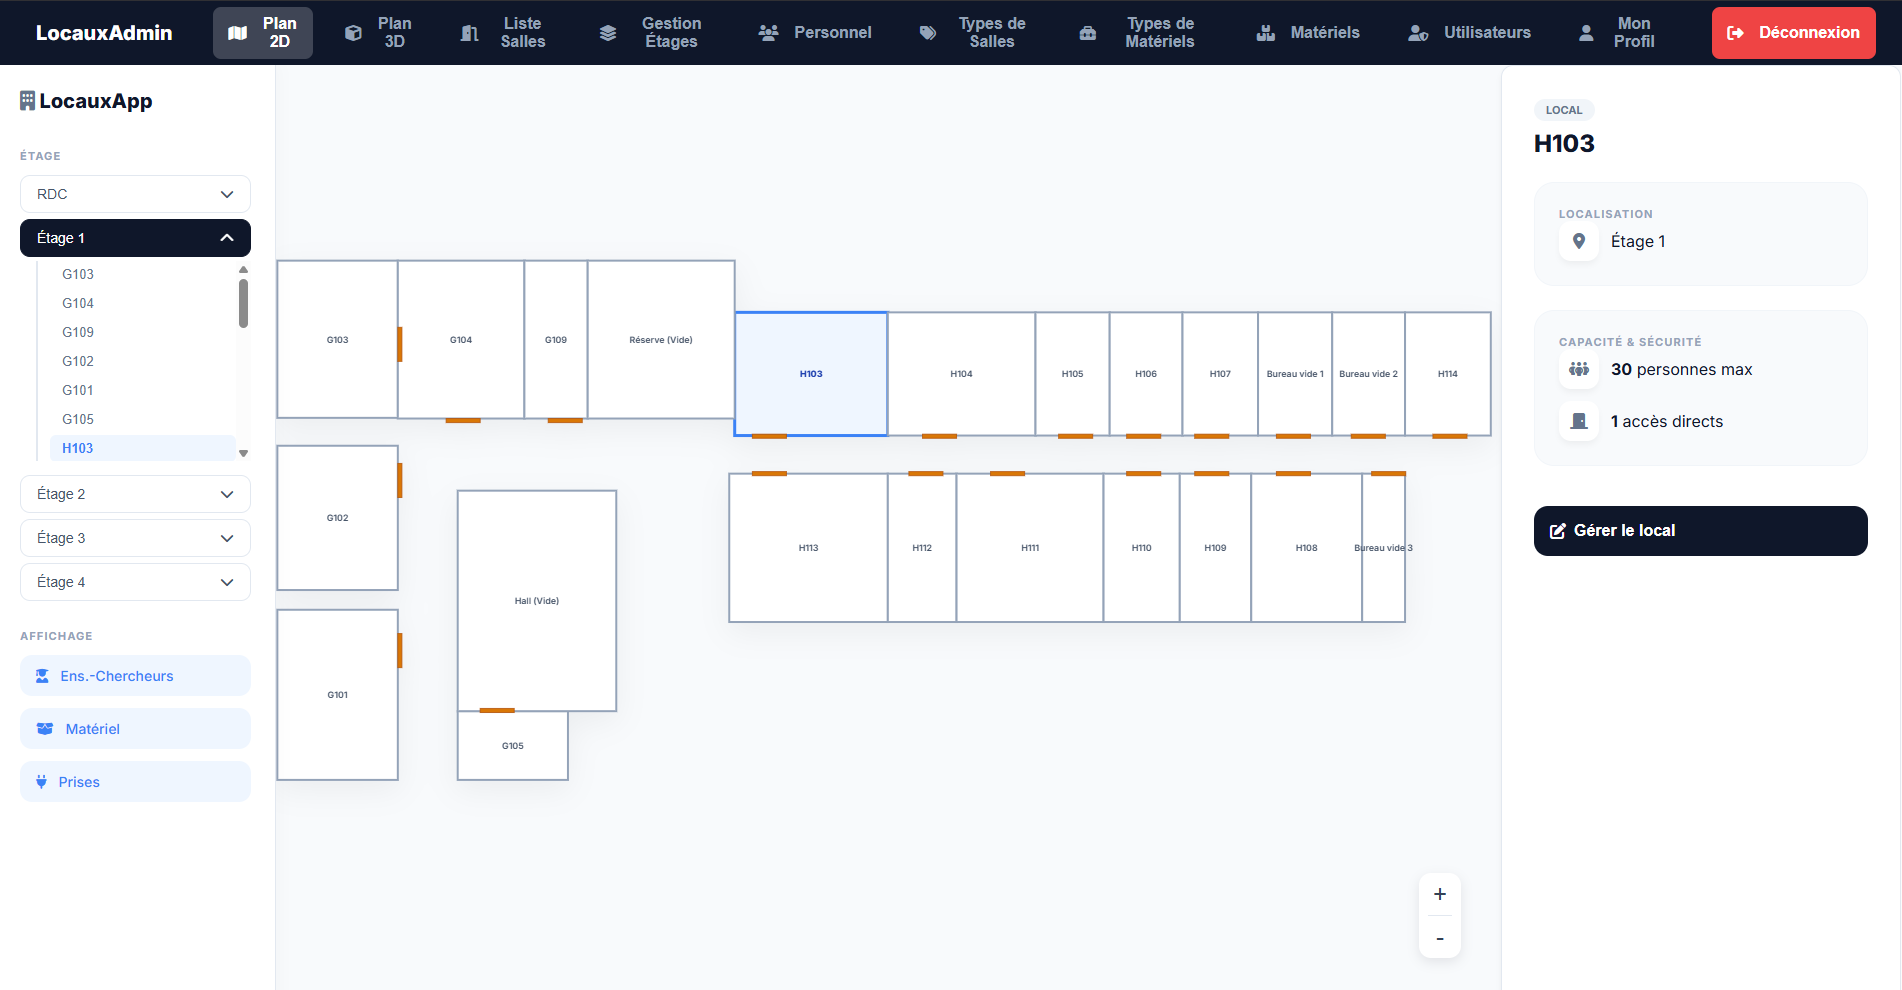
\includegraphics[width=\linewidth,keepaspectratio]{img/screenshot_interface.png}
    \caption{Interface de visualisation des plans JSON avec options d'export PDF}
    \label{fig:screenshot-interface}
\end{figure}
